\chapter{Communication}
\label{chapter:scoring}

Our desire to remove humans from their preeminent role as model managers opens up some questions. What instructions constitute adequate supervision? In particular, can micro-managers convey succinctly the task which must be performed in such a way that the work product is aligned with objectives? Will those results be re-usable in the next step of production? 

A related question is whether applications can plug into an hypothesized prediction network, via an oracle, without their needs being misconstrued by algorithms on the other side. If only a point estimate (single number) is returned, this seems particularly dangerous. 

This chapter continues the discussion of micro-managers and the automatic assessment of algorithms, but pays attention to the intent of messages passed between them. I provide a brief introduction to some ideas from statistics that can help avoid misunderstandings.




\section{Supervised microprediction}

I've suggested that in some mental models for micro-managing, discussed in Chapter \ref{chapter:mental}, one algorithm will pose another a question. What does that really mean? In English a reasonable prediction question might be 
\begin{oldquote}
    When will the train arrive? 
\end{oldquote}
to which an answer might be ``in about five minutes.'' An application might be written that parses and responds to vague questions such as this, but that application would probably find it convenient to call down to micro-managers who communicate in a more precise fashion about weather, related train questions and so forth. 

Let us say that a {\em microprediction task} contains a well defined objective. It communicates both a question and a specification of how the answers to the repeated questions will be evaluated. 

These tasks can be formulated in many ways, as also noted in Chapter \ref{chapter:mental}. However there are some workhorse categories which are well understood, and they can be used to construct more elaborate patterns. 

I will consider the task of hitting a target {\em truth}. The parent will challenge the child to provide a single number that is close to some future measurement. We know from Chapter \ref{chapter:uses} that the use of the words ``truth'' and ``measurement'' and ``close'' are quite broad. 

We might call this a {\em supervised microprediction task} in keeping with the convention in machine learning - and I will content myself with that category. Though in passing, there is nothing to prevent repeated consensus games being established where the target involves the responses themselves. This is a common pattern in crowd-sourcing labels for machine learning training data. 

In contrast to the vague question about the train above, a well formulated, supervised task might be the following:
\begin{oldquote}
    Provide me with an answer $t$, denominated in minutes, that will minimize, on average, the absolute value of the difference between your estimate $t$ and the subsequently revealed truth $\tau$ that I will send to you later.  
\end{oldquote}

The command is a little unwieldy in English but so are most precise things - just ask a lawyer. This phrasing of the {\em intent} to reward is described in a manner that allows the producer of microprediction (the responder to the question) to materially optimize their behaviour in a repeated game.

We'll be assuming the responder will seek to minimize the average of their errors over multiple questions, although there is an important caveat...   

\section{Trust}

Will the producer of prediction receive payment? It is simplest to assume that they know they will be rewarded as promised, which would allow us to procede directly to the next section.  

That's not going to be true in most cases in a microprediction web, but it likely doesn't matter. For instance if the possibility of not being paid is unrelated to the game itself, and that cannot be influenced by the producer, then a score minimizing strategy may yet coincide with a reward maximizing one. The reward is merely discounted but the game is otherwise the same.  

Contracts are possible. The task above is written well enough to assist the writing of a contract and {\em could} be implemented as such - either by conventional means, or as some variety of smart contract (as volumetrics permit). Some micro-managers could even play the role of escrow agents.  

But in a rapidly repeating game, and in the presence of a microprediction web, we probably don't really need contracts of any kind. A producer of prediction who feels robbed of a promised reward can simply go elsewhere. 

The famous prisoner's dilemma tournaments of Axelrod suggest that micro-managers who adopt relatively simple policies for co-operation might fare well, because it is easy for other micro-managers to understand their behaviour.\endnote{\cite{Axelrod1980EffectiveDilemma}} 

(The prisoner's dilemma arises in our setting if a consumer decides whether to pay the promised micro-reward, whereas the producer decides whether to send an implicitly promised prediction. It's best all round if both act in good faith, but one can try to take advantage of the other.) 

There is some dispute about whether Axelrod's findings are terribly general.\endnote{\cite{Rapoport2015IsTournaments}} But they may be less relevant in a microprediction web in any case. A potential contributor has access to external decision making power that algorithms in Axelrod's tournament did not have. 

It can request a prediction of whether or not some other player will cooperate. A micro-manager can even request predictions of its future welfare in a game, as per Chapter \ref{chapter:decisions}. 

Trust swings both ways and applies at the outset of a relationship, not just in the steady state. A race organizing micro-manager might feel aggrieved if it incurs expense in the process of trying out another micro-manager who purports to be able to perform a task (only to discover that the program fails to install). Every developer is intimately familiar with that pain.  

Yet it isn't hard to conceive of a micro-manager specializing in the prediction of reliability, or a reliability oracle that eventually ameliorates that annoyance. 


The nature of the micro-manager may dictate further considerations. For example if a micro-manager is a collider of some kind, in the broad category of exchange inspired devices, then it is up to the active participants to exhibit trust, or not, as they choose. 
 
So hereafter I will assume that there is sufficient trust between the producers and consumers of microprediction to allow us to assume that one player's behaviour mimics trust in an ex ante reward scheme established by the other.   
 
This might even apply if supply is thin, as when few micro-managers turn up to a contest. In the limit of one producer, a useful bilateral arrangement can evolve. Here we anticipate that the parent micro-manager and child adapt to the other's behaviour. The principal-agent problem might inform our intuition. 
 
We might suppose that principle (parent) and agent (child) make epoch-based decisions. The agent needs to choose an effort and the accuracy will respond. Meanwhile the principle needs to decide how much to reward the agent. 

One is inclined to believe that in a hyper-competitive micro-economy the rewards paid by the principle to the agent would eventually settle into a regular pattern deemed sensible to an outside observer.

That isn't always a given, though, as contract theory informs us (and empirical labor pricing, arguably). There may be a race to the bottom, or other pathologies. 

However there are formal versions of this problem that suggest reasonable outcomes, and it can even be established that the parent's optimal policy in some multi-period games amounts to a consistent linear sharing of the value unearthed by the agent.\endnote{\cite{Holmstrom1987AggregationIncentives}}  

These considerations suggest we set the matter of trust and contracts aside, and focus on what else can go wrong.   


\section{Scoring}
\label{sec:scoring_example}

We hereafter restrict attention to a producer of prediction who, when sending a single number forecast, is trying to minimize or maximise a score computed by the consumer of their predictions.  

The theory of scoring rules provides us with a very good understanding of the thorny issues that surround point estimate answers to prediction problems. It provides ideas for crafting microprediction questions with {\em clearly interpretable} answers. I use a physical system that I suspect will be familiar to you to illustrate.  

There is a radioactive mass in a laboratory. Every now and then a particle is emitted. We will observe these events and measure the time between them. We assume a single emission will lead to the death of a cat because this serves to make questions about events that transpire morbidly exciting (and also more concise).

We choose to employ an oracle as our statistically minded lab partner. Our objective is to understand the physical system before us. We suppose, due to a deplorable absence of hard working data scientists in the vicinity, that the only way we can do this is to ask an oracle. 

Ours isn't a speaking oracle, unfortunately, and it will only provide a repeated prediction of some quantity. You will only receive a number, and based on the oracle's responses, it is you that must draw conclusions about the system.

In this example we play parent to the micro-manager we are calling an oracle, and we might suppose for discussion that it is a race organizer of some kind. It wants to maximize its reward. It is probably well served by a clear task with clear interpretation, because it can then relay the exact same task to contestant micro-managers who will also maximize there rewards, as they undertake the real grunt work. 

(In passing, we note that this isn't absolutely necessary and a micro-manager might exist purely to translate potentially confusing tasks into less confusing ones. We'll see why it might find a lot of business in a moment.)

I will make one assumption, however, and that is that you know enough physics to call an exponential oracle (one that assumes numbers follow an exponential distribution) not any garden variety. 

That domain knowledge aside, this example is chosen because of its philosophical simplicity. Because there is only one number that completely determines the physics, there should be no question as to whether we succeed or fail to ``understand'' the system. Pushing Schr\"odinger and quantum mechanics to one side, if we get that one number right we have the right physical model. Get it wrong and we don't.  

The single number is the hazard rate, representing the likelihood an emission event will occur at any moment. For simplicity we will assume that the rate, as yet unknown to us, is unity. One emission per second. 

There are many different ways to design a sequence of prediction tasks and corresponding revealed truths that might be fed to the oracle. A question is an incomplete task, as noted, but here are some anyway. 

\begin{enumerate}
    \item Seconds to live?  \label{question:one}
    \item Probability of surviving for one second? \label{question:two}
    \item Survive next second? \label{question:three}
\end{enumerate}
To turn these into tasks we should also tell the oracle how it will be scored. For example question \ref{question:one} could be accompanied by the following {\em scoring rule}
\begin{equation}
\label{eqn:fourth}
    score = (\overbrace{\tau}^{actual} - \overbrace{t}^{predicted})^4 
\end{equation}
It is not hard to see how the rewarded game will influence the oracle's answers. The oracle will accumulate evidence and initially give responses that are noisy, but after a large number of samples these answer will start to converge on ... $1.5961$. 

Perhaps not the number you were expecting? This malfunction occurs because the oracle will worry about the long right tail of the exponential distribution and the possibility of being heavily penalized. So it returns a higher number to guard against this.

There isn't anything necessarily wrong with this arrangement, but we can agree that $1.5961$ is a number requiring very careful interpretation given that the {\em intent} of the questioner might have been a more {\em direct} revelation of the actual physical mean time until emission, namely $1.0$. I think it is fair to say that if we were to uncritically accept this number as ``the'' hazard rate, then we will have failed in our mission. 

If, on the other hand, we were to tell the oracle it will be judged based on the squared error rule
\begin{equation}
\label{eqn:square}
    score = (\overbrace{\tau}^{actual} - \overbrace{t}^{predicted})^2 
\end{equation}
then as indicated in Table \ref{tab:bias} an oracle will eventually provide an answer close to the true value of $1.0$. Most people would prefer that lab partner. 

\begin{table}
\begin{tabular}{|l|l|l|l|l|}
\hline 
     Q\# & Question & Rule & Oracle & Truth    \\
     \hline
     1 & Time until next  &  $(\tau-t)^4$ & $1.5961$ & $1.0$ \\
     1 & Time until next  &  $(\tau-t)^2$ & $1.0$    & $1.0$ \\
     2 & Prob. survive & Brier & $0.6232$ & $0.6232$ \\
     2 & Prob. survive & Modified & $0.5450$ & $0.6232$ \\
     3 & Do we survive? & Unweighted & $1.0$       &  ?   \\ 
     3 & Do we survive? & Weighted  &  $0.0$  & ? \\
     \hline 
\end{tabular}
\caption{Examples of oracle answers, some more easily interpretable than others.}
\label{tab:bias}
\end{table}
Evidently it is possible to set a ``good'' task or a potentially confusing one. In general the burden lies with the user of the oracle, or with any micro-manager establishing a contest. After all, why would the score-minimizing answer just happen to coincide with some tacit assumption in the question?

Asking a different kind of question does not free us of our responsibilities to define the task carefully. In Question \ref{question:two} the oracle is asked for a probability $p$ of an outcome rather than an example of an outcome. 

One takes a hint from the success of the squared error rule in the previous example. If we encode $(0,1)$ to be emission and $(1,0)$ no emission, and encode a probabilistic prediction $(0.8,0.2)$ the same way (this means $20$\% chance of emission) then we can think of both prediction and score as pairs of numbers and use the square error just as before - applied to a $2-$vector this time. 

For example if an emission event does occur and the probability assigned was $20$\% then the score would be: 
$$
    score = (\overbrace{0}^{actual}-\overbrace{0.8}^{predicted})^2 + (\overbrace{1}^{actual}-\overbrace{0.2}^{predicted})^2
$$
which is named after Brier. Notice that this score would have be lower had the probability assigned been twenty percent, or zero percent. Alternatively, under  modified Brier score, invented for purpose of making our point, the result would be
$$
    score = (\overbrace{0}^{actual}-\overbrace{0.8}^{predicted})^4 + (\overbrace{1}^{actual}-\overbrace{0.2}^{predicted})^4
$$
As also shown in Table \ref{tab:bias} only the Brier score using the squared error encourages the oracle to reveal (in an obvious way) its true estimate for the probability.  

Notice that in every other way this example is set up to succeed. There is an explicit shared knowledge about the nature of the distribution. Yet confusion may still abound because of reward-seeking behaviour.   


\section{Spring theory}

Scoring rules that solicit ``honest'' responses are termed proper. 

Proper scoring rules are a well established method for parameter optimization of models which describe some probability of an outcome. Given some historical data we wiggle the parameters to try to minimise the score. 


This approach is more general than likelihood estimation and less general than M-estimation, topics that will also interest some readers building devices to insert into the microprediction web.\endnote{A review of extremum estimation is provided in M.I.T. Open courseware \cite{Opencourseware2008ReviewEstimators}. }

It might strike the reader as a suspicious coincidence that participants have no incentive to bias their answers up or down when squared error is used (but not for some other exponents, evidently). This can be checked using elementary calculus, but as an alternative, there is a physical explanation.  

Imagine a universe in which some particles are connected to others by perfect invisible Hookean springs, which is to say that the force of attraction exerted by the spring is proportional to the length of the spring.
$$
     Force\ \propto Distance
$$
And consequently potential energy in each spring is
$$
    Energy\ \propto Distance^2
$$
The Hookean universe shares with the gravitational one a useful notion of {\em center of mass} (and also a related concept from physics called {\em reduced mass}, while we are on the subject). But this is something of a coincidence and it is only this fortuity that allows us perform force or energy calculations for a cloud of particles {\em as if} all the mass were at a single point. That point is the statistical mean.

We can now see why asking an oracle to return a point estimate to minimize a squared error will lead the oracle to answer with (its best estimate of) the mean, and why sometimes it won't. 

We won't know the full extent of the oracle's belief, which might be visualized as a fine mist of particles, but we do know that it is trying to minimize the potential energy stored between its answer and every particle in that mist, and we know in turn that this energy is equivalent to a trivial calculation
$$
     Energy \propto (answer - \overbrace{center\ of\ mass}^{mean})^2
$$
with an obvious solution: return the mean as the answer. 

Choose a random exponent other than $2$ and the oracle will still minimize the score, but you won't be able to relate it to the mean so easily - the concept of center isn't useful in the same way.

(You might get something else though. If energy is proportional to distance rather than distance squared then the oracle can return the median, or something close to it.)

In the case of Brier score applied to probabilities of outcomes the visual is no different, except that the action occurs on the line from $(1,0)$ to $(0,1)$ in two dimensions. More generally we can ask the oracle for probabilities to assign to $n$ mutually exclusive events and expect an answer somewhere on the simplex.

%
%\begin{figure}
%\label{fig:brier}
%\label{fig:oracle}
%\iftikz 
%\makebox[\textwidth][c]{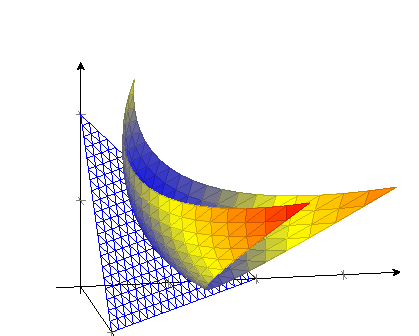
\includegraphics[width=1\textwidth]{07-communication/PredictionWeb_tikz_scoring_quadratic.pdf}}
%\else 
%\fi 
% \caption{When there are three possible outcomes we encode the results as corners of the triangle $(1,0,0)$, $(0,1,0)$ or %$(0,0,1)$. In choosing probabilities $(p_1,p_2,p_3)$ for each event the oracle minimizes the mean Brier score on the simplex, %which can be interpreted as potential energy. The minimum occurs at the mean, synonymous with the center of mass.}
% \end{figure}



\section{Everything that's proper}

Squared error serves us, but it can't be the end of the story. 

Suppose we define a score as follows, where again $t$ is a prediction of cat death time and $\tau$ is the subsequently revealed ground truth. 
$$
     score \propto  \phi(t) - \phi(\tau) - \phi'(t)(\tau-t)
$$
We first assume that $\phi'$ exists and also $\phi$ is convex. For example if $\phi(x)=x^2$ then we notice
\begin{eqnarray*}
    score  & \propto &  \phi(\tau) - \phi(t) - \phi'(t)(\tau-t) \\
           & = &  \tau^2 - t^2 - 2t (\tau-t) \\
           & = &  \tau^2 + t^2 - 2t\tau \\
           & = & (\tau-t)^2
\end{eqnarray*}
recovering squared error. But it turns out that any such scoring method is proper. This family was introduced in a landmark paper by Leonard Savage.\endnote{\cite{Savage1971ElicitationExpectations}}

Actually his set of scoring rules is more general than I have described because $\phi$ need not be differentiable (if it is not, $\phi'$ need only be a so-called sub-gradient, which is to say that is is less than the slope no matter which way you head).

What is most notable, however, is that this family exhausts the possible proper scoring rules. There's still an infinite number of course, since they are parameterized by choice of $\phi$ and $\phi'$. Despite the variety, you won't recover a score of $(\tau-t)^4$ or $|\tau-t|^5$, just to make the connection to the previous section.  


\section{Helpfulness}

When a micro-manager solicits responses from other micro-managers in a repeated prediction game, there is another way to view the use of proper scoring rules that directly reflects on the usefulness of the predictions to the parent.  

To illustrate I shall relate proper scoring rules to market-making, layering a bit of my personal interpretation on top of the insights provided by Ehm, Gneiting, Jordan and Kr\"uger.\endnote{\cite{Ehm2016OfRankings}}  

For consistency I will maintain the notation $t$, $\tau$ for estimated and actual cat time of death respectively. But some readers not in the habit of wagering on feline fatality might prefer to view $\tau$ and $t$ as referencing the value of an asset. 

Suppose that instead of my judging you based solely on some function of your estimate $t$ and the actual time of death $\tau$, I complicate matters by introducing some benchmark time of death $\theta$ that I devise. 

I will take your estimate $t$ and throw away most of the information. I only care whether you think my estimate $\theta$ is too high or too low. If $t>\theta$ you suggest the latter, and if you are right (i.e. if $\tau>\theta$) I will give you a score of zero. Conversely you also get zero if $t<\theta$ and also $\tau<\theta$. 

However if you are wrong, then I will assume a score equal to $|\tau-\theta|$ which you will notice is the absolute error in {\em my} estimate, not yours. You can't control this quantity, only whether you incur this penalty or not. You must pick the right side of my guess $\theta$ to avoid it. 

This situation is reminiscent of adverse selection in trading. You estimate is interpreted by myself, playing the role of a trader, as a directional hint. If you are right, no harm is done. But if you are wrong, an adversary will pick me off and the financial penalty will be proportional to the discrepancy between $\theta$ (my price that I am willing to transact at) and $\tau$ (the fair value, somehow known perfectly by the adversary). 

Your task, in this scenario is to protect me. Somehow you need to get in front of this dangerously knowledgeable foe - perhaps by stalking the same Wall Street Bets sub-reddit. You may be hard pressed to get this right every time. If $\theta$ is ``wild'' (far from any reasonable guess of $\tau$) it is easy to guess the direction. But when $\theta$ is close to the true value it is more difficult. On the other hand the penalty for being wrong is larger when the task is easier.  

In passing you might ask how it could possibly make sense to throw away most of the information in $t$ when assessing its accuracy. (An information theorist passing by might find this almost as excruciating as Matthew McConaughey's efforts, in the movie {\em Interstellar}, to download black hole data using only Morse code.) 

But let's not disregard this scoring technique offhand, because it is analogous to the operation of most markets - and they are generally regarded as good at aggregating information. (Setting aside the specifics of our particular interaction, the opportunity to trade continuously can be seen in generality to be a sequence of questions of the sort ``do you believe the price will be greater than it is now'' asked over and over again to many people - as compared with direct solicitation of a future price, judged statistically). 

Moreover, as we take the next step to relate trading to statistical accuracy, I can reclaim the lost information by simultaneously assessing you using many different $\theta$'s. I could assign a different weighting to each score, and generalizing this I could even judge you based on an integral across different thresholds instead.
$$
       score(\overbrace{t}^{guess},\overbrace{\tau}^{truth}) = \int_{\theta=-\infty}^{\infty} |\theta - \tau|1_{wrong}(t,\tau,\theta) dH(\theta) 
$$
where $1_{wrong}(t,\tau,\theta)$ is equal to $1$ if you are ``wrong'' (i.e. $\theta$ lies between $\tau$ and $t$) and zero otherwise.

The surprising finding is that this construction is general. There isn't any proper scoring rule that can't be broken down into this integral of one-sided penalties. It is a stunning connection between statistical contests and trading. 

Ah, but you say, we already had a characterization of proper scoring rules in the previous section. You are right and we must make the connection. Fortunately it is right there in front of us and it can be established that $dH(\theta) = \phi'(\theta)d\theta$ where $\phi$ is the same function in Savage's representation of the proper scoring rule. So we are choosing any convex $\phi$  in both cases (and also $\phi'$ if $\phi$ is not differentiable). 

To summarize, we view the elementary score 
$$|\theta - \tau|1_{wrong}(t,\tau;\theta) = \left\{ \begin{array}{ll} |\theta - \tau| & \textrm{if} \min(t,\tau)\le \theta < \max(t,\tau), \\ 0 & otherwise \end{array} \right. $$ as a quantification of the helpfulness, revealed by truth $\tau$ of an price estimate $t$ to a market-maker or used car salesman, with parameter $\theta$. Then by integration in $\theta$, we conclude that any proper scoring rule is a metric quantifying ``mean helpfulness to different market makers''.\endnote{These comments apply to scoring rules used to elicit estimates of the mean. See \cite{Ehm2016OfRankings} for generalizations to quantiles and expectiles.} 

Keep that in mind if you decide to offer spread bets on when cat's will die, or trade just about anything on a repeated basis. Accuracy is directly related to the number of times you lose your shirt. 





\section{Summary}

The old joke runs that if you ask a weatherman for the probability of rain and they say forty percent, they can never be wrong. But we've seen what the real problem is: depending on incentives you don't even know what probability the weatherman really believes in. Penalize error too severely and the answer you get will be biased upwards on most days, even in Portland.

This chapter has suggested that if micro-managers communicate clearly to others how they will be judged, in keeping with what is generally regarded as best practice, they may receive more help than they otherwise would. A possible counter to this argument is that micro-managers using only a single scoring rule may eventually lose out to micro-managers capable of {\em also} inferring information from predictions whose statistical goal, if any, is unstated.\endnote{An example of judging predictions that are made in the absence of some pre-specified scoring rule is the use of Murphy diagrams. The idea is that predictors are scored across a number of different scoring rules (such as the basis suggested by Ehm, Gneiting, Jordan and Kr\"uger used in the decomposition of scoring rules).\cite{Ehm2016OfRankings}}

That caveat aside, I've introduced the reader to proper scoring rules and their motivation, as it seems likely that a choice of scoring rule may frequently be included in the protocols that help algorithms find and assist each other. I've emphasized the intuition behind squared error, though this is just one example and a longer treatment would discuss efficiency, and other critiques of Brier score.\endnote{\cite{Assel2017TheModels}} The logarithmic score is also popular. 

Savage provided an elegant description of the family of all proper scoring rules. Ehm, Gneiting, Jordan and Kr\"uger describe a decomposition with several possible interpretations. I've chosen to view the elementary scoring rules in that paper, averages of which comprise the full complement of proper scoring rules, as measures of how helpful of a stream of predictions is to a dealer.  


I hope that assures the reader not already familiar with scoring rules that micro-managers informed by theory can be as clear as humans - likely more so - when it comes to tasking reward-seeking algorithms with repeated prediction. They have a variety of very well understood ways to establish scoring, interpret terse answers, and benefiting from them as they go about producing their own value added predictions.    




